\section{Calibration using a photometric correction}% {\color{YellowGreen} Laurence} }
\label{se:photocorr_calibration}

As discussed in Sect.~\ref{se:obsdate_variations}, observations during the
afternoon sessions or
%the morning session after observations close to the direction of the
%Sun
during sunrise are deeply affected by the \afternoon\ beam
size variations, which are either due to solar irradiation
of the primary mirror and anomalous atmospheric refraction
(afternoons) or to a focus drift (sunrises).
For the baseline calibration presented in
Sect.~\ref{se:baseline_calibration}, this effect was mitigated by
discarding the scans acquired during these periods, as defined by the
baseline selection of Sect.~\ref{se:data_selection}. However, in
this section, we address the issue of calibrating in presence of
\afternoon beam variation effect. We discuss a
calibration method that relies on a photometric correction
depending on the beam size. 

When using the photometric correction, no scan selection based on the
observation date is performed. However, the scans from which the
absolute calibration is derived, are selected on the FWHM estimate
using the same criteria as for the baseline calibration, that are FWHM
thresholds of $12.5''$ at 1mm and $18''$ at 2mm.  Thus, only
the scans that are moderately affected by the beam effect are included
in the absolute calibration in order not to include twice the
photometric correction uncertainties in the error budget (once for the
absolute calibration and once for the photometry).

% ALL METHOD RESULTS 
\begin{table}[!thbp]
\begin{center}
\begin{tabular}{|c|l|c|c|c|c|c|}
  \hline
  \multicolumn{2}{|c|}{}  &  \multicolumn{5}{|c|}{Methods} \\\cline{3-7}
  \multicolumn{2}{|c|}{Characteristics} &  baseline  & taumeter  &  skydip  &  photocorr demo & photocorr pointing \\
  \hline\hline
   \multicolumn{2}{|c|}{$\#$ selected scans} & 26    &       26  &    26    &    38           &    38 \\ 
  \hline 
  Factor &  A1          &   1.00  &  0.97   &  1.13    &   1.01    &   1.02  \\
       &  A3            &   1.00  &  0.97   &  1.02    &   1.01    &   1.00  \\
       &  1mm           &   1.00  &  0.95   &  1.06    &   1.01    &   1.01  \\
       &  2mm           &   1.00  &  0.94   &  0.99    &   1.01    &   1.01  \\
  \hline
  RMS  &  A1            &  3.2    &   4.2   &   3.4    &    3.5    &   3.0 \\
  $[\%]$     &  A3            &  3.6    &   4.3   &   3.3    &    3.5    &   3.0 \\
       &  1mm           &  3.3    &   4.5   &   3.3    &    3.1    &   2.6 \\
       &  2mm           &  1.6    &   2.6   &   1.5    &    1.5    &   1.5 \\
\hline\hline
\end{tabular}
\caption[Comparison of calibration results using five methods]{Comparison of calibration results using five methods}
\label{tab:Abs_calibration_results_all}
\end{center}
\end{table}

\subsection{Photometric correction methods}
\label{se:photocorr_methods}

When the beam size broadens due to e.g. \afternoon\ beam effect, the
flux density is smeared in a larger solid angle and
the flux density estimator, which is based on the amplitude fit of a
Gaussian beam of fixed FWHM as described in
Sect.~\ref{se:flux_density_equation}, is biased toward low flux densities.

Considering only the main beam broadening, modeled as a Gaussian of
size $FWHM' = 2 \sqrt{2\ln{2}} \, \sigma '$, we show in
Sect.~\ref{se:photometric_correction} that
the flux density estimator depends on the size of the convolution
function between the enlarged $\sigma '$-Gaussian\samu{, which can be
  monitored as in Sect.~\ref{se:obsdate_variations}}, and the 
$\sigma_0$ fixed-width Gaussian of our reference system. An unbiaised
flux density $\hat{S}_{pc}$ can be derived from the flux density
estimate $\hat{S}$ as
\begin{equation}
  \hat{S}_{pc} = f(\sigma')\hat{S},
\end{equation}
where $f(\sigma')$ is a photometric correction of the beam variation
effect. Within the Gaussian model, it reads:
\begin{equation}
  f(\sigma') = \frac{(\sigma'^2 + \sigma_0^2)}{\sigma_{\star}^2 + \sigma_0^2}. 
\end{equation} 

The beam size in stable observing condition $\sigma_\star$ is
determined by measuring the 2D Gaussian beam on the series of scans of
source with various flux density, which has been used for the beam
characterization in Sect.~\ref{se:MB}.
An empirical model for the small correlation of
$\sigma_\star$ with the source flux density is given in
Sect.~\ref{se:photometric_correction}.

The photometric correction thus relies on the measure of the current beam
size $\sigma'$. The induced uncertainties on the flux density
measurements depends on the precision of which we are able to monitor
the beam size. 

We perform two case studies: \new{the paragraph titled ``Demonstration case''} presents a demonstration
calibration assuming the beam is precisely monitored, whereas
the ``Practical case using pointing scans'' paragraph addresses a practical calibration relying
on a beam monitoring using pointing scans. 

\subsubsection{Demonstration case}
\label{se:photocorr_demo}

For the demonstration case, shortened as 'demo' hereafter, we use a
photometric correction based on the Gaussian FWHM fitted on the map
of the source. This method thus applies only on point-like
sources that are bright enough for an accurate fit of the beam to be
obtained using a single scan.  

The beam size is estimated by fitting a 2D Gaussian from the map and
forming the geometrical $\sigma$,
$\sigma_{\rm{geom}} = (\sigma_x \sigma_y)^{1/2}$\new{, where
  $\sigma_x$ and $\sigma_y$ are the 2D Gaussian standard deviation
  along the $x-$ and $y-$axis respectively.}

In order to capture only the beam size variations driven by the
observing conditions (primary mirror deformations, anomalous
refraction, elevation), a small correction $\delta_{\rm{geom}}$ has to be made to
the 2D Gaussian beam FWHM estimate for bright sources. The estimate of the
actual Gaussian size $\sigma '$ is
\begin{equation}
  \hat{\sigma '} = \sigma_{\rm{geom}} - \frac{\delta_{\rm{geom}}}{2\sqrt{2 \ln{2}}}, 
\end{equation} 

where the offset $\delta_{\rm{geom}}$ is null for faint or moderately
bright point sources, and non-zero for bright sources.
As for $\sigma_\star$,  the 2D Gaussian fit yields slightly broaden
$\sigma_{\rm{geom}}$ for bright sources (e.g. planets) to accomodate
for the side lobes, which are measured with high signal-to-noise.
For Uranus, $\delta_{\rm{geom}}$ includes also the beam widening due
to Uranus disc, which is seen with a diameter of about $3.5''$ at the
IRAM 30-m telescope latitude. We measure Uranus $\delta_{\rm{geom}}$
by comparing the average $\sigma_{\rm{geom}}$ estimates using Uranus
scans and using MWC349 scans, we found $\delta_{\rm{geom}} = 0.4''$ at
1-mm and $\delta_{\rm{geom}} = 0.25''$ at 2-mm, which basically
distributes as one half being due to Uranus finite extension and the
other half stemming from the side lobes. 
%, in consistency with
%the empirical $\sigma_\star$ variations with flux discussed in
%Sect.~\ref{se:photometric_correction}.


\subsubsection{Practical case using pointing scans}
\label{se:photocorr_pointing}

For sources fainter than about one Jy, the signal to noise ratio is in
general not high enough to allow for a precise measure of the beam to be
made from a single observation scan, so that the 'demo' is not
usable. Ideally, dedicated scans must be made in order to accurately
monitor the beam variations, e.g. a few minute duration OTF scan on a
pointing sources every 30 or 60 minutes. These scans are not available
yet. However, here we propose and test the use of the \emph{pointing} scans
themselves to monitor the beam.

The pointing scans, which are described in Sect.~\ref{se:pointing},
are used to estimate pointing corrections during observations. As they
consist of two sub-scans in azimuth and elevation of about 10 seconds
of integration time each, they can be used to project a map of the
pointing source. The beam size is estimated by fitting a 2D Gaussian
and forming the geometrical FWHM, labeled $FWHM_{\rm{p}}$. No
significant offset is observed for bright sources because, unlike maps
based on OTF scans, \new{pointing scan maps have a low signal-to-noise
ratio that prevents the geometrical FWHM from being sizably affected by the
side lobes.}
However, the beam widening due to the apparent diameter has been taken
into account in the case of Uranus.
As a summary, for the pointing-based photometry correction method,
shortened as 'pointing' hereafter, the
beam variations are monitored using the estimate of the
actual Gaussian size $\sigma '$ 
\begin{equation}
  \hat{\sigma '} = \sigma_{\rm{p}} - \frac{\delta_{\rm{p}}}{2\sqrt{2 \ln{2}}}, 
\end{equation} 
where $\sigma_{\rm{p}}$ is the geometrical $\sigma$ corresponding to
$FWHM_{\rm{p}}$ and the offset $\delta_{\rm{p}}$ is null for
point-like sources and equals to $0.2''$ at $1\,\rm{mm}$ and $0.13''$
at $2\,\rm{mm}$
for pointing scan of Uranus. The beam variation monitoring using
pointing scans has been detailed in
Sect.~\ref{se:obsdate_variations}.



\subsection{Stability against observing conditions}

Here we check the stability of Uranus measured-to-predicted flux
density ratio against the beam size and the atmospheric transmission
when using a photometric correction for the beam variations.
The measured flux density relies on the 'corrected skydip' opacity
measurements to correct for the atmospheric attenuation.  

First, we present Uranus flux density ratio as a function of the beam FWHM
after the photometric correction with the 'demo' and 'pointing'
methods in the fourth and fifth row panels of
Fig.~\ref{fig:calib_uranus_vs_fwhm_all} respectively. The flux density
is stable against the beam FWHM within rms errors for both
wavelengths. In addition, more scans are used for the absolute
calibration, as also reported in
Table.~\ref{tab:absolute_calibration_scan_numbers}, including scans
acquired in the early afternoon.

\begin{figure}[!htbp]
\begin{center}
  % corrected skydip
  \begin{overpic}[clip=true, trim={0, -0.3cm, -0.3cm, 0}, width=0.35\textwidth]{Figures/Calibration/plot_flux_density_ratio_obstau_uranus_corrected_skydip_narrow_1mm.pdf}
    \put(20,23){\footnotesize Baseline}
  \end{overpic}
  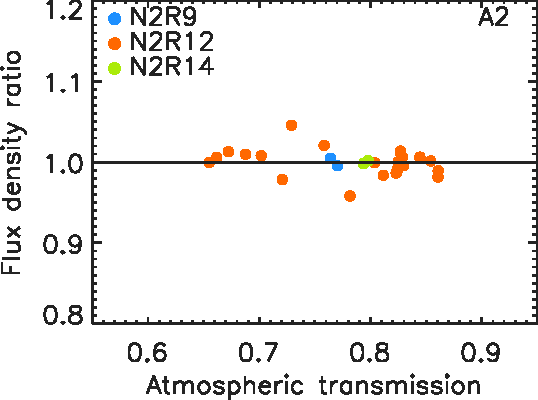
\includegraphics[clip=true, trim={0, -0.3cm, -0.3cm, 0}, width=0.35\textwidth]{Figures/Calibration/plot_flux_density_ratio_obstau_uranus_corrected_skydip_narrow_a2.pdf}
  % taumeter
  \begin{overpic}[clip=true, trim={0, -0.3cm, -0.3cm, 0}, width=0.35\textwidth]{Figures/Calibration/plot_flux_density_ratio_obstau_uranus_tau225_narrow_1mm.pdf}
    \put(20,23){\footnotesize Taumeter}
  \end{overpic}
  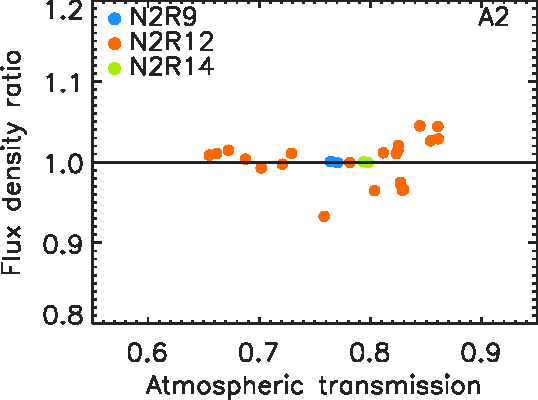
\includegraphics[clip=true, trim={0, -0.3cm, -0.3cm, 0}, width=0.35\textwidth]{Figures/Calibration/plot_flux_density_ratio_obstau_uranus_tau225_narrow_a2.pdf}
  % skydip
  \begin{overpic}[clip=true, trim={0, -0.3cm, -0.3cm, 0}, width=0.35\textwidth]{Figures/Calibration/plot_flux_density_ratio_obstau_uranus_skydip_narrow_1mm.pdf}
    \put(20,23){\footnotesize Skydip}
  \end{overpic}
  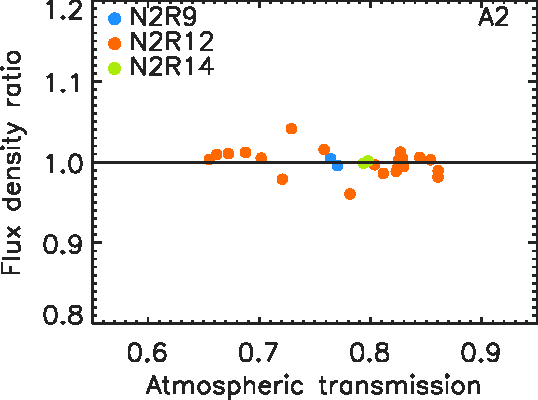
\includegraphics[clip=true, trim={0, -0.3cm, -0.3cm, 0}, width=0.35\textwidth]{Figures/Calibration/plot_flux_density_ratio_obstau_uranus_skydip_narrow_a2.pdf}
  % corr. sky. photocorr demo
  \begin{overpic}[clip=true, trim={0, -0.3cm, -0.3cm, 0}, width=0.35\textwidth]{Figures/Calibration/plot_flux_density_ratio_obstau_uranus_corrected_skydip_photocorr_demo_narrow_1mm.pdf}
    \put(20,23){\footnotesize Photocorr Demo}
  \end{overpic}
  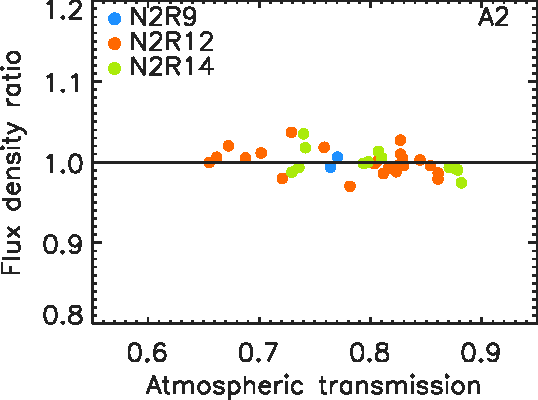
\includegraphics[clip=true, trim={0, -0.3cm, -0.3cm, 0}, width=0.35\textwidth]{Figures/Calibration/plot_flux_density_ratio_obstau_uranus_corrected_skydip_photocorr_demo_narrow_a2.pdf}
  % corr. sky. photocorr pointing
  \begin{overpic}[clip=true, trim={0, -0.3cm, -0.3cm, 0}, width=0.35\textwidth]{Figures/Calibration/plot_flux_density_ratio_obstau_uranus_corrected_skydip_photocorr_pointing_narrow_1mm.pdf}
    \put(20,23){\footnotesize Photocorr Pointing}
  \end{overpic}
  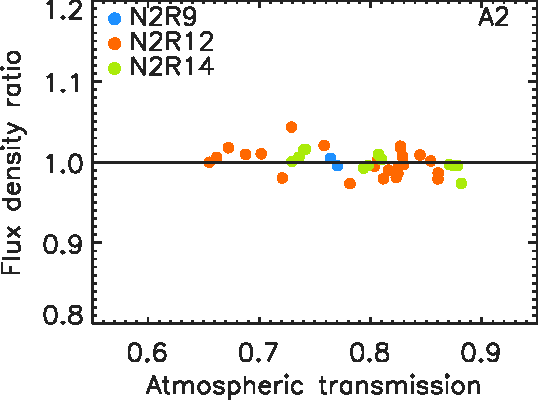
\includegraphics[clip=true, trim={0, -0.3cm, -0.3cm, 0}, width=0.35\textwidth]{Figures/Calibration/plot_flux_density_ratio_obstau_uranus_corrected_skydip_photocorr_pointing_narrow_a2.pdf}
  \caption[Uranus flux density stability against atmospheric
    transmission]{Uranus flux density ratio vs atmospheric transmission
    shown for the $1$-mm array
    combination (left column) and for array 2 (right column) after absolute
    calibration using (\emph{first row}:) the baseline method, as
    well as (\emph{second row}:) the 'taumeter'-based and
    (\emph{third row}:) the 'skydip'-based methods, and methods
    relying to (\emph{fourth row}:) the 'demo' and (\emph{fifth
      row}:) the 'pointing' photometric corrections. These plots
    include all Uranus scans acquired during N2R9, N2R12 and N2R14
    campaigns. }
  \label{fig:calib_uranus_vs_atmtrans_all}
\end{center}
\end{figure}


In Fig.~\ref{fig:calib_uranus_vs_atmtrans_all}, we check the stability
of Uranus flux density ratios against the atmospheric transmission using
the 'demo' (fourth row) and 'pointing' (last row) photometric
corrections. The atmospheric transmission model and the colour
conventions are the same as in Sect.~\ref{se:baseline_calibration_atm}.
The flux ratios at both wavelengths are consistent with the
unity within statistical errors for the whole tested range of
atmospheric transmissions using both the 'demo' and the 'pointing'
photometric correction. Average absolute calibration factors normalised
to the baseline calibration factor, as well as the \new{relative} rms errors are
gathered in Table~\ref{tab:Abs_calibration_results_all} in the columns
labeled 'photocorr demo' and 'photocorr pointing'. We find that,
resorting to a photometric correction i) allows us to use $45\%$ more
scans for the absolute calibration, ii) has a negligeable impact on
the absolute calibration factor and iii) yields a small reduction of
the flux density ratio dispersion. For the absolute calibration, the
'pointing' photometric correction performs as well as the 'demo' case.
Photometry capability and stability when using a photometric
correction will be further tested in Sect.~\ref{se:photometry_others}. 





